\documentclass[11pt]{article}
\usepackage[margin=0.8in]{geometry}
\usepackage{graphicx} % Required for inserting images
\setlength{\parindent}{0pt}
\usepackage{float}
\usepackage{caption}

\title{{\fontsize{21pt}{18pt}\selectfont COL216 Lab Assignment - 0} \\ Variable Latency Multiplier}
\author{Yash Bansal \\ 2022CS511333 \and Shivam Sawarn \\ 2022CS1107}
\date{}
\begin{document}

\maketitle

\section{Problem Statement}

\begin{enumerate}
    \item Implement a fixed-latency fixed-point multiplier in VHDL to multiply two 16-bit unsigned binary numbers.
    \item Enhance the multiplier using Booth's multiplication algorithm to create a variable-latency multiplier. Compare the performance of the two algorithms for multiple random inputs.
\end{enumerate}

\section{Design Principles}

\subsection{Adder}

Initially, a 16-bit adder circuit was designed to serve as a component in the multiplier circuit. The design incorporates principles from both carry-lookahead adder and ripple carry adder methodologies:

\begin{itemize}
    \item Four full-adder circuits, each of 4 bits, are designed. A carry-lookahead adder is employed to maintain the carry, with the initial carry of the 1st adder set to 0.
    \item Following the ripple carry adder principle, the carry of the 1st adder ripples to the 2nd adder and so on until the outputs of all four adders are computed.
    \item The final carry, denoted as \texttt{c\_out}, is stored as part of the output signal.
\end{itemize}

\subsection{Fixed-point Multiplier}

In the fixed-point multiplier, the following steps are done until our variable cycle is 16:

\begin{itemize}
    \item The variable cycle represents the position of the multiplier bit and the corresponding position of the addition in the result. The result is initialized as a 32-bit vector (\texttt{c\_1075}) with all bits set to '0'.
    \item If the current multiplier bit is '0', the algorithm moves to the next bit without computation, taking one clock cycle.
    \item For the case when the multiplier bit is '1', an additional variable \texttt{cycle2} is introduced. When \texttt{cycle2} is '0', a required 16-bit number is extracted from \texttt{c\_1075} and added to the multiplicand. After this, \texttt{cycle2} is set to '1'.
    \item When \texttt{cycle2} is '1', the result of the addition (computed from \texttt{cycle2 = '0'}) is assigned back to \texttt{c\_1075} at the appropriate position, making it a two-clock cycle operation for cases where the multiplier bit is '1'.
    \item When the variable cycle reaches 16, the final result is computed and stored in the vector \texttt{c\_1075}.
\end{itemize}

\begin{figure}[H]
  \centering
  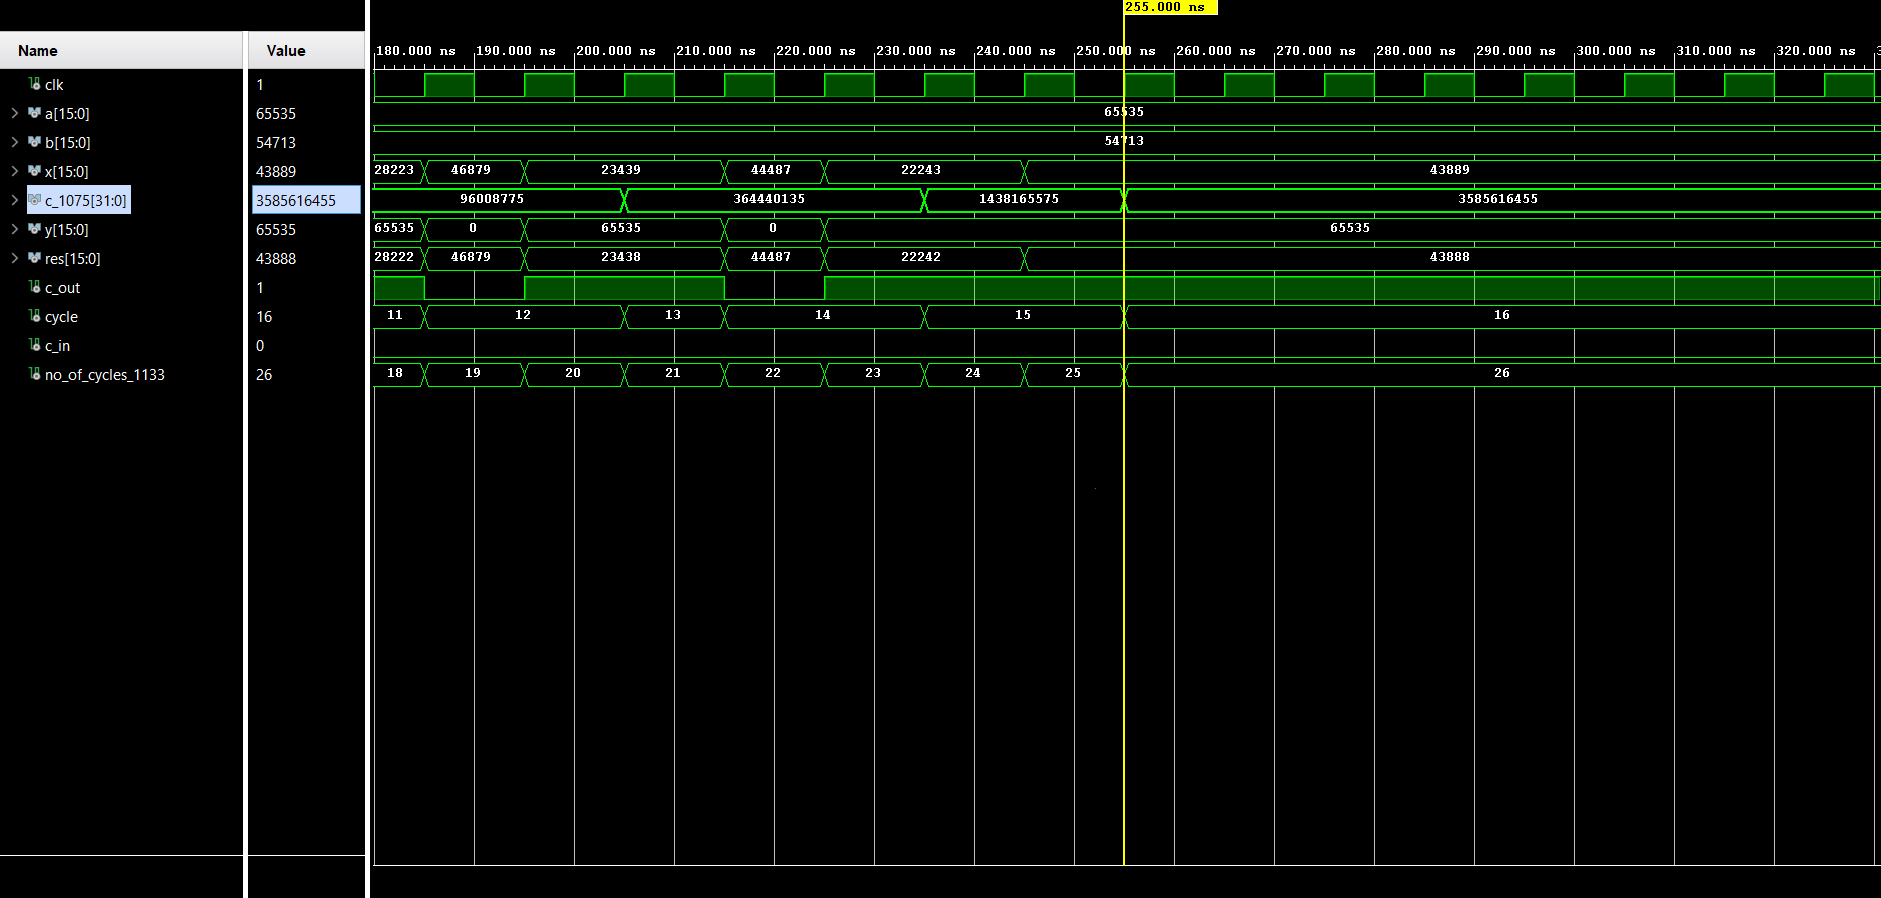
\includegraphics[width=1\textwidth]{img1.png}
  \captionsetup{labelformat=empty}
  \caption{a(multiplicand) = 65535 \ \ \ \ \ \ \ \ \ \ \ \ \ \ \ \ \ \ b(multiplier) = 54713 }
  \caption{c\_1075(final result) = 3585616455 \ \ \ \ \ \ \ \ \ \ \ \ no\_of\_cycles\_1133 = 26 \ \ \ \ \ \ \ } 
\end{figure}

\subsection{Subtracter}

A 32-bit subtracter is designed to be utilized as a component for Booth's multiplication algorithm:

\begin{itemize}
    \item Similar to the adder circuit, a 4-bit carry-lookahead adder and ripple carry adders are combined, with the initial carry set to '1'.
    \item Before the subtraction operations, the bits of the second number are inverted to represent its 2's complement form.
\end{itemize}

\subsection{Booth's Multiplier}

In Booth's multiplier, the following steps are performed for a variable cycle count of 17:

\begin{itemize}
    \item Two variables, \texttt{c} and \texttt{d}, each of 32 bits, are created and initialized to 0. The final answer is stored in \texttt{final\_res\_1075}.
    \item When the current multiplier bit is '1' and the previous bit is '0', an additional variable \texttt{cycle2} is used. When \texttt{cycle2} is zero, a required 16-bit number is extracted from the vector \texttt{d} and added to the multiplicand. After this, \texttt{cycle2} is assigned '1'. When \texttt{cycle2} is '1', the result of the addition is assigned back to \texttt{d} at the appropriate position. The vector \texttt{d} represents the sum of all the numbers subtracted in Booth's algorithm.
    \item When the current multiplier bit is '0' and the previous bit is '1', a similar process is followed with \texttt{c} representing the sum of all the numbers added in Booth's algorithm.
    \item The final result is obtained by subtracting \texttt{c} and \texttt{d}, and the result is stored in \texttt{final\_res\_1075}.
\end{itemize}

\begin{figure}[H]
  \centering
  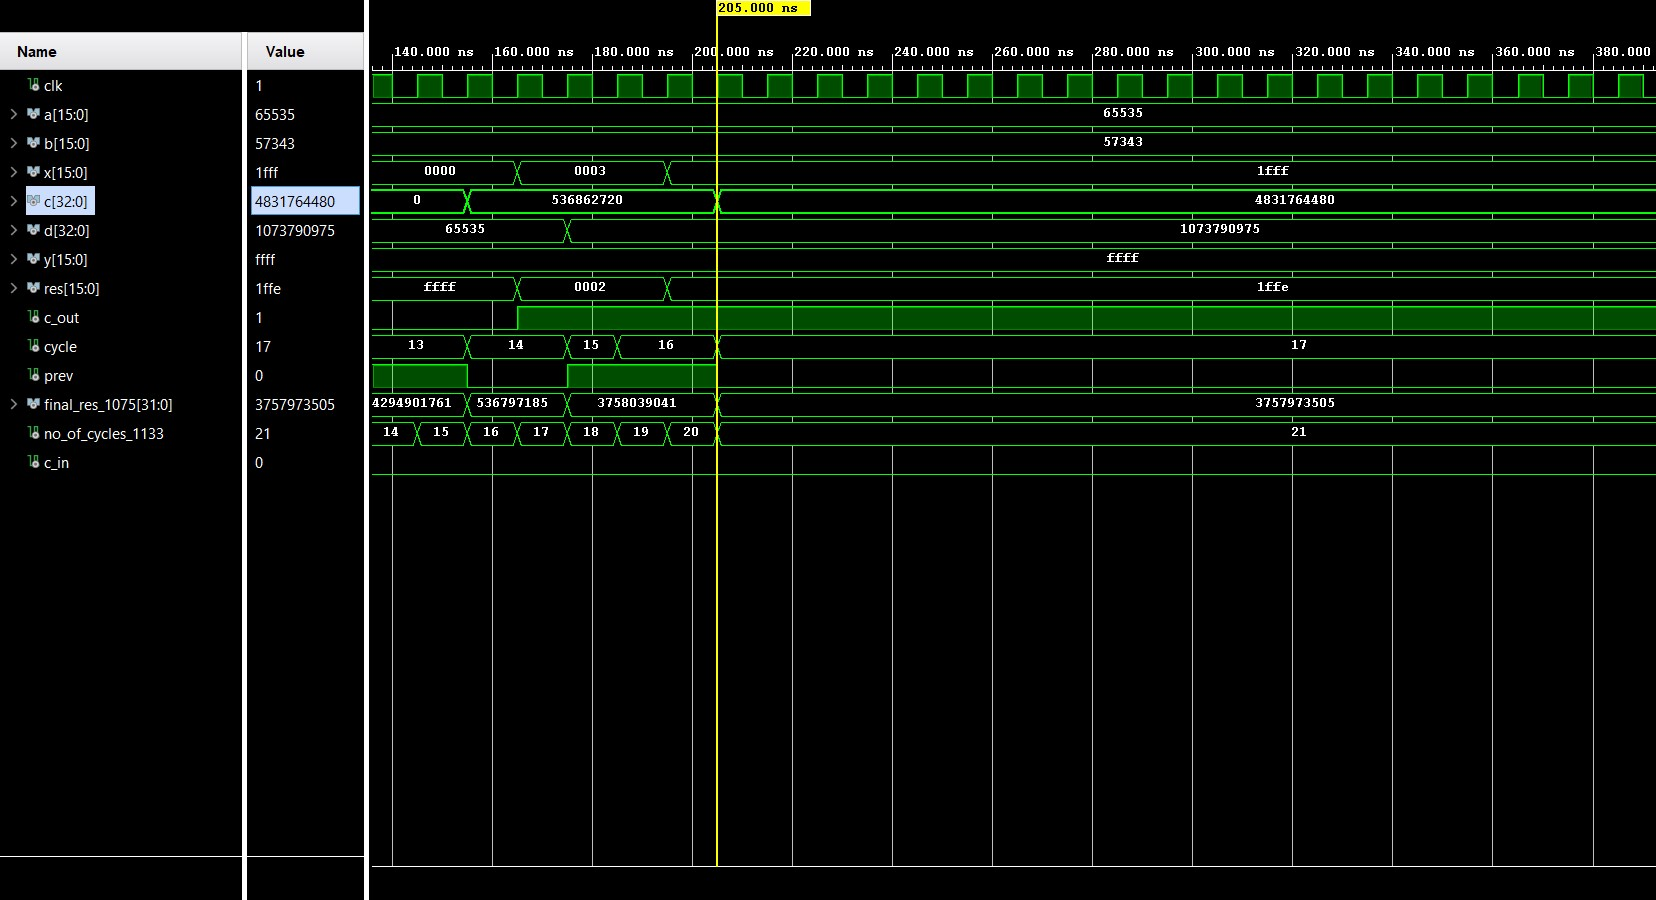
\includegraphics[width=1\textwidth]{img2.jpg}
  \captionsetup{labelformat=empty}
  \caption{a(multiplicand) = 65535 \ \ \ \ \ \ \ \ \ \ \ \ \ \ \  \ \ \ \ \ \ \ \ \ \ \ \ \ \ \ \ \ \ \ \ \ b(multiplier) = 57343 }
\caption{c(booth\_addition) = 4831764480 \ \ \ \ \ \ \ \ \ \ \ \ \ \ \ \ \ \ d(booth\_subtraction) = 1073790975 }
  \caption{final\_res\_1075(final result) = 3757973505 \ \ \ \ \ \ \ \ \ \ \ \ \ \ \ \ \ \ \ \ \ \ no\_of\_cycles\_1133 = 21 \ \ \ \ \ \ \ \ \ \ \ \ \ \ \ \ } 
\end{figure}

\section{Note:-}
\begin{itemize}
    \item 
main2.vhd is implementation of fixed-point multiplication and main3.vhd is the implementation of booth multiplier.
\end{itemize}
\end{document}
